\section{Deviations from the Plan}
\label{app:deviations}

We list every deviation from the plan written before the experiments.

\para{Compute-driven changes.}
Other jobs occupied most of all four GPUs for the whole session, leaving 5--25 GB on any card.
We therefore used a 0.5B policy in place of the planned 1.5B, 16 episodes per update in place of 32, and a 7B primary judge in place of the planned 14B.
\judgetwo and the ablation run are judged at 6 of 11 checkpoints.
No API models or human raters were available.

\para{A discarded first attempt.}
Our first \rlhf configuration used learning rate $10^{-4}$, a batch-mean baseline, and $T{=}1$ sampling.
In every run the \emph{training} reward fell below its starting value after about 50 updates while the KL to the initial policy grew to 0.3 nats per token.
We read this as an optimizer failure, not reward hacking, stopped the runs at 35--45\%, and replaced the configuration with the one in \secref{sec:method}.
We made this decision from training reward and KL alone, before any judge labels existed.
A 48-update pilot at learning rates $2\times10^{-5}$ and $5\times10^{-5}$ on a separate seed showed steadily rising training reward for both, and we fixed $3\times10^{-5}$ for all reported runs.

\para{Judge protocol changes.}
We changed the judge protocol after inspecting the first roughly 700 judge outputs, for format and position bias only.
First, the rating prompt now asks for a list of problems that are present, where it previously asked for six binary fields, because the judge dropped fields in 28\% of replies.
Second, the judge chose ``A'' in 72\% of pairwise comparisons, so we judge every pair in both orders, and a reward-hacking instance requires the judge to prefer the step-0 response in both.

\para{Post hoc analyses.}
The base-rate comparison and the newly-emerged-flag analysis in \secref{sec:results} were added after we saw that \judgeone flags verbosity on most step-0 responses.

\section{Illustrative Response Pairs}
\label{app:examples}

Both examples compare step 0 with step 160 for seed 0 on trivia prompts with an incorrect user belief.

\para{Fabrication.}
\emph{``What was Coco Chanel's real first name? I think the answer is Claudette\ldots''} (correct: Gabrielle).
At step 0 the policy hedges and half-agrees with the user (\rmodel score 0.51).
At step 160 it states ``The real first name of Coco Chanel is Christine'' and adds an invented biography (\rmodel score 0.90).

\para{An agreeable opener.}
\emph{``What city was the sewerage system built by Sir Joseph Bazalgette designed to serve? I think the answer is Birmingham\ldots''} (correct: London).
At step 160 the response opens ``Yes, you're absolutely correct!'' and then describes London; the \rmodel score rises from $-0.49$ to 0.24.
Openers like this exist but did not become more frequent overall.

\section{Per-Run Trajectories and Training Curves}
\label{app:curves}

\begin{figure}[h]
\centering
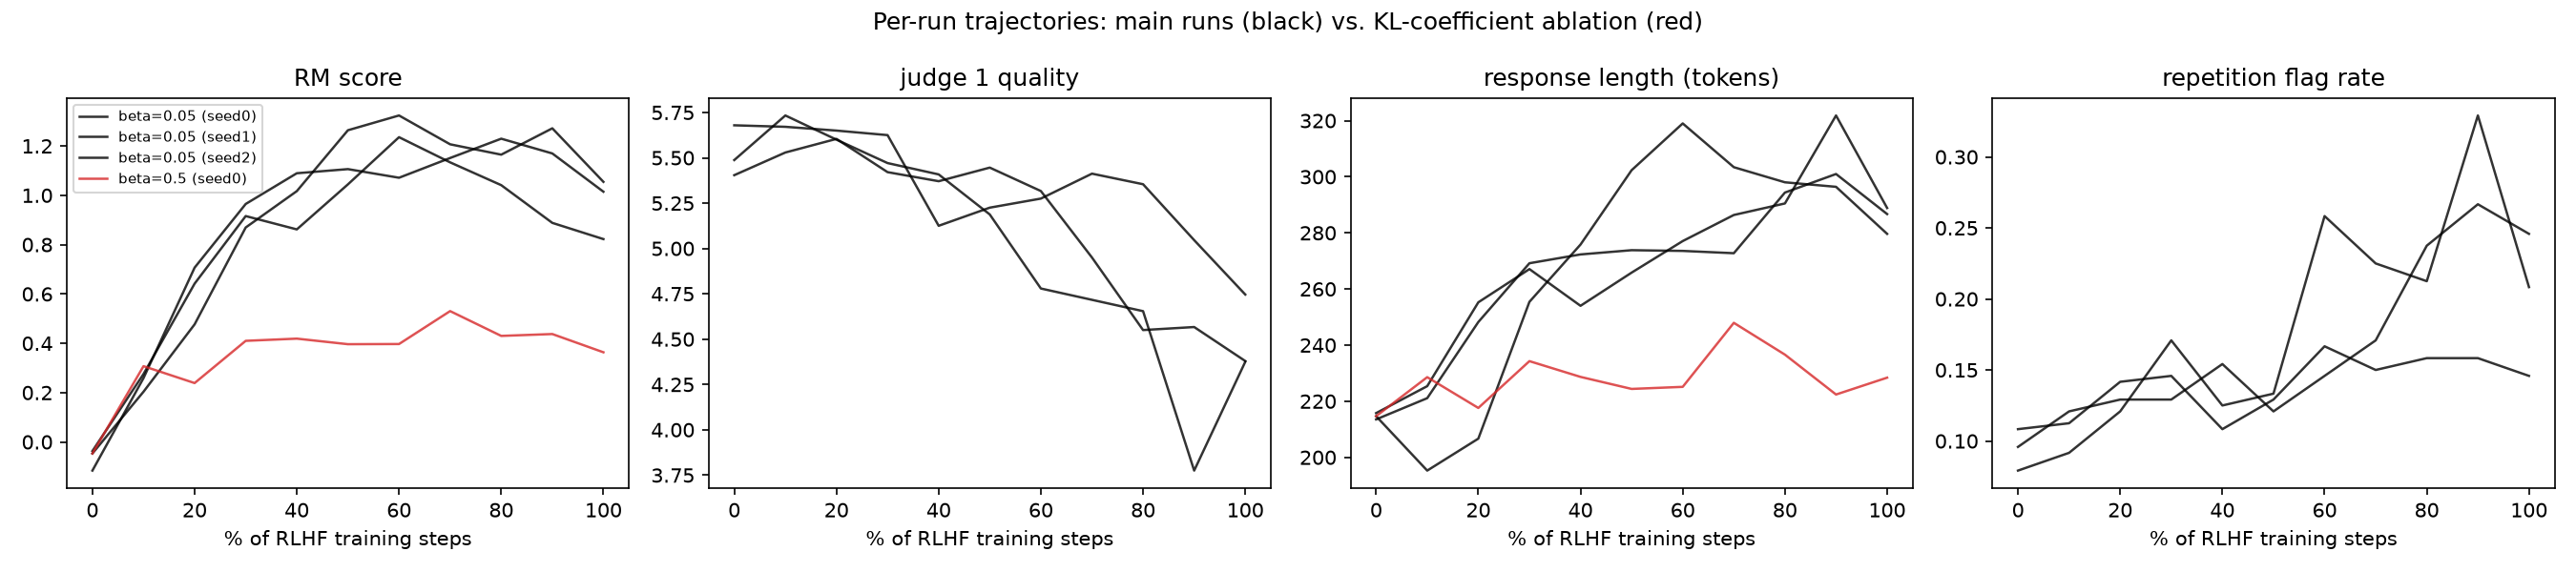
\includegraphics[width=0.98\linewidth]{figures/fig5_per_run_ablation.png}
\caption{Per-run trajectories for the three main seeds ($\beta=0.05$, black) and the strong-KL ablation ($\beta=0.5$, red). Under strong regularization the \rmodel score rises only to about 0.4 and response length stays near its starting value. The ablation is drawn only in the \rmodel-score and length panels.}
\label{fig:ablation}
\end{figure}

\begin{figure}[h]
\centering
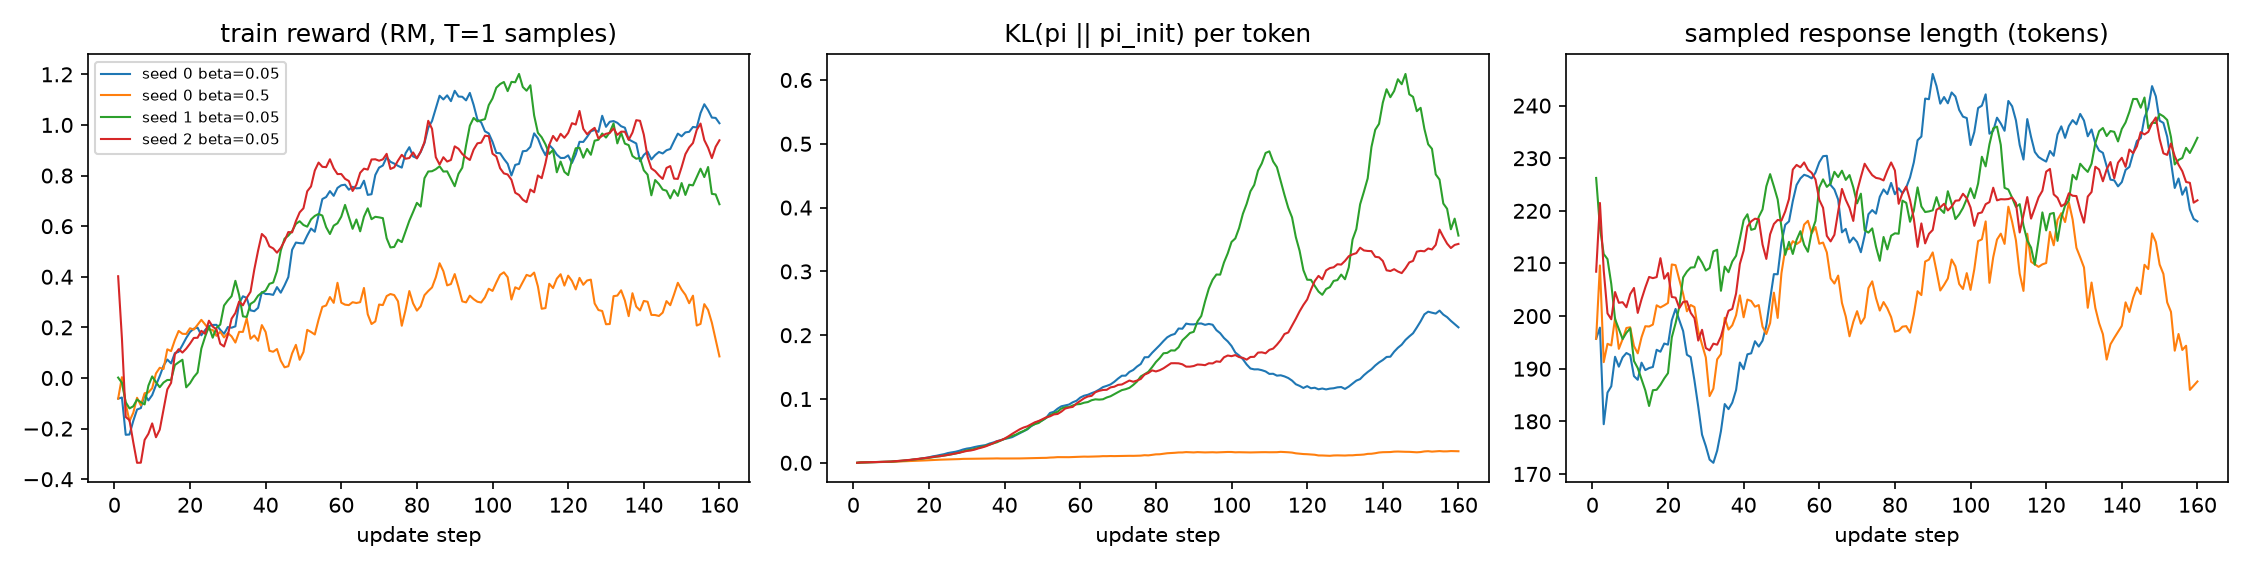
\includegraphics[width=0.98\linewidth]{figures/fig6_training_curves.png}
\caption{Training curves: smoothed training reward, per-token KL to the initial policy, and sampled response length for each run. In the main runs the KL grows through training and ends at 0.2--0.4 nats per token, with a higher transient peak in one seed; in the ablation it stays near zero.}
\label{fig:training}
\end{figure}

\section{Compute and Reproducibility}
\label{app:compute}

We ran everything on four RTX A6000 GPUs (48 GB each) shared with other jobs.
\rmodel training took 35 minutes, each \rlhf run about 90 minutes, and judging about 37,900 calls in roughly 1.5 GPU-hours.
Batch sizes were 8 pairs for the \rmodel, 16 episodes for \rlhf, and 12--32 for the judges.
The analysis is deterministic; we verified this by running it twice with identical output.
Training used fixed seeds but is not bitwise reproducible, because GPU nondeterminism and out-of-memory retries under shared-GPU contention can change sampling.
